\documentclass[border=10pt]{standalone}
\usepackage{tikz}
\usetikzlibrary{arrows.meta, shapes, calc}

\begin{document}
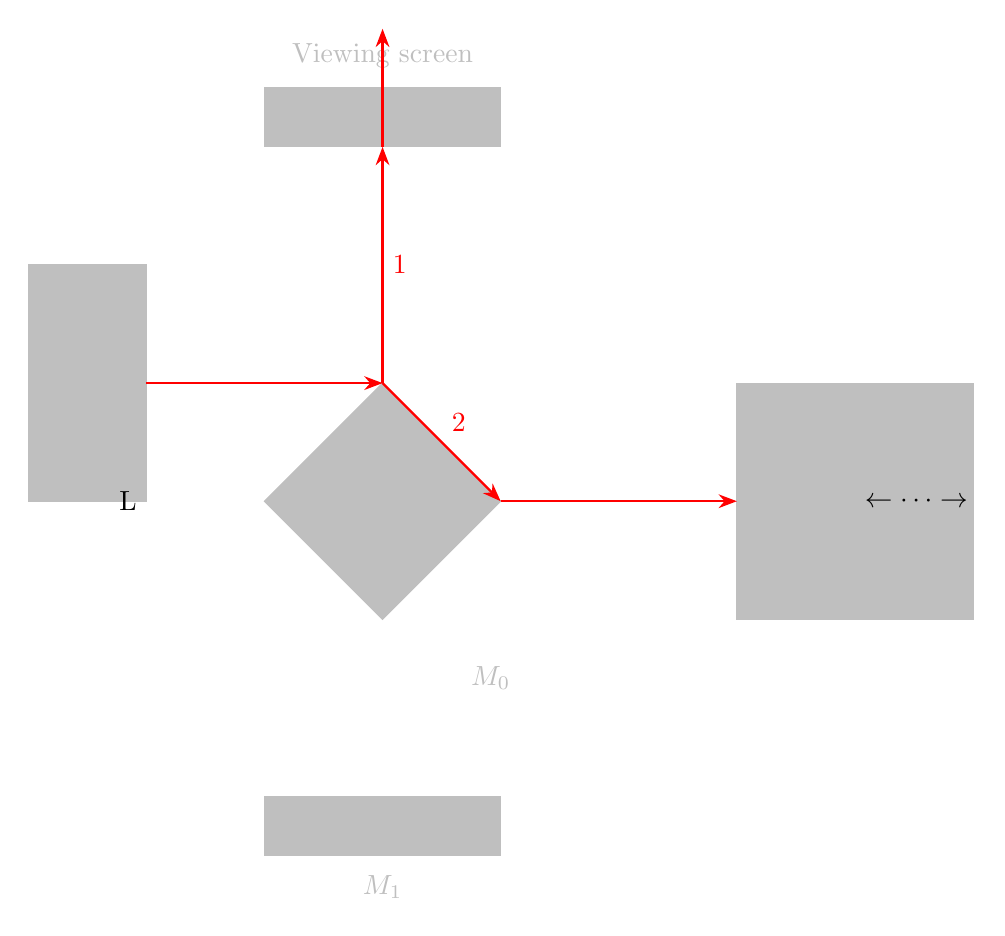
\begin{tikzpicture}[scale=1.5, >=Stealth]

% Components
\filldraw[gray!50] (-3,0) rectangle ++(1,2) node[midway] {L};
\filldraw[gray!50] (0,-1) -- (1,0) -- (0,1) -- (-1,0) -- cycle node[right=1cm] {$M_0$};
\filldraw[gray!50] (-1,-3) rectangle ++(2,0.5) node[midway,below=0.5cm] {$M_1$};
\filldraw[gray!50] (3,-1) rectangle ++(2,2) node[midway,right=0.5cm] {$M_2$};
\filldraw[gray!50] (-1,3) rectangle ++(2,0.5) node[midway,above=0.5cm] {Viewing screen};

% Light Paths
\draw[red, thick, ->] (-2,1) -- (0,1);
\draw[red, thick, ->] (0,1) -- (1,0) node[midway, above right] {2};
\draw[red, thick, ->] (1,0) -- (3,0);

\draw[red, thick, ->] (0,1) -- (0,3) node[midway, right] {1};
\draw[red, thick, ->] (0,3) -- (0,4);

% Labels
\node at (-2,0) [left] {L};
\node at (4,0) [right] {$\leftarrow \cdots \rightarrow$};

\end{tikzpicture}
\end{document}